\newpage
\chapter{Lung Ultrasound Protocols}
Lung ultrasound (LUS) is used in different healthcare settings, including low- to middle-income countries, where access to advanced imaging technologies like computed tomography (CT) may be limited. Therefore, researchers developed protocols to use of pulmonary ultrasound in clinical settings in a easier way. 

\section{The BLUE Protocol}
Among the most commonly adopted is the BLUE (Bedside Lung Ultrasound in Emergency) protocol \cite{lichtenstein2008blue}, established by Lichtenstein and his team, which is widely used by healthcare professionals to help diagnose the underlying causes of acute respiratory failure.

BLUE were initially intended to be straightforward and fast to diagnose the causes of acute respiratory failure in clinical settings. It was assumed that when acute respiratory failure occurred, the lungs, being such a huge organ, would reveal broad and readily observable diseases. Conditions like pulmonary edema, pulmonary embolism, pneumonia, chronic obstructive pulmonary disease (COPD), asthma, and pneumothorax can be identified using specific profiles outlined in the BLUE protocol. During COVID-19 this protocol became obsolete, since performing a 6-points lung ultrasound exam may miss lung pathology related to COVID-19.
\begin{figure}[h]
    \centering
    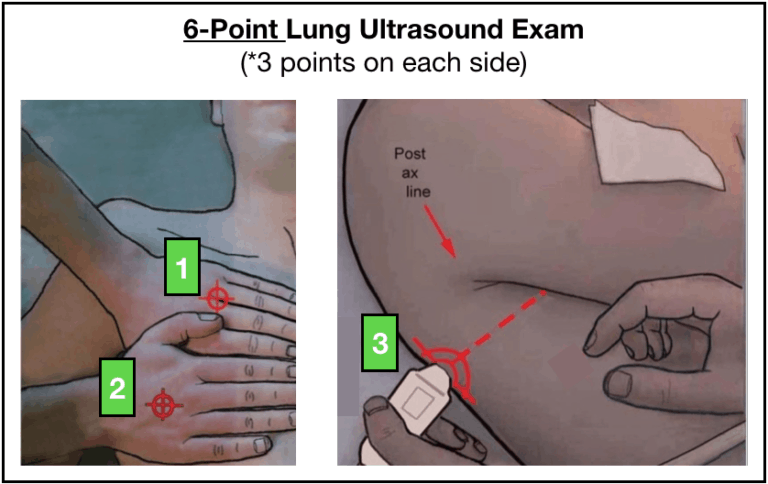
\includegraphics[width=0.5\linewidth]{images/us_protocols/6-points-protocol.png}
    \caption{6-points protocol (3 for each side) of BLUE}
    \label{fig:enter-label}
\end{figure}
\section{The new 12-Points Protocol}
Soldati et al. \cite{soldati2020proposal} presents a comprehensive framework aimed at optimizing the use of LUS in the diagnosis and management of COVID-19 employing a 12-points protocol. The authors highlight the  role of LUS as a diagnostic tool, expecially in the context of the COVID-19 pandemic as it is capable of detecting various lung conditions. Some of these are lung disease and acute respiratory distress syndrome, which are critical in managing COVID-19 pneumonia.
The authors pointed out the need for a unified approach, hence the team has developed a standardized protocol for its use in COVID-19 management.
This protocol includes specific recommendations regarding the equipment used, such as the adoption of wireless transducers and tablets.
These choices are made to minimize the risk of contamination during examinations, which is particularly important in the context of infectious diseases. 
By establishing a standardized method, the authors aim to ensure consistency in LUS practices across different healthcare settings.
 A significant contribution of the article is the introduction of a scoring system designed to classify the severity of lung involvement in COVID-19 patients based on LUS findings. This scoring system was developed through a collaborative effort involving the review of a substantial number of anonymized cases. By categorizing the severity of lung conditions, clinicians can make more informed decisions regarding patient management and treatment strategies, ultimately leading to better patient care.
The authors advocate for the establishment of an international database dedicated to sharing LUS images and videos to facilitate the collaboration among healthcare professionals and researchers worldwide. By pooling resources and knowledge, the medical community can enhance the development of pattern recognition algorithms and improve telemedicine capabilities. Such collaboration is crucial in a global health crisis, as it allows for the rapid dissemination of best practices and findings. The article provides practical guidelines for conducting LUS examinations effectively. Key recommendations include avoiding the use of cosmetic filters and specific imaging modalities that may obscure important findings. The authors stress the importance of achieving high frame rates during imaging to capture subtle lung changes accurately. Additionally, they recommend saving data in the Digital Imaging and Communications in Medicine (DICOM) format or as video files to ensure that visual findings can be reviewed comprehensively. With respect to the acquisition, 14 areas should be scanned per patient for 10 seconds. The areas are divided in this way:
\begin{itemize}
    \item 3 lateral
    \item 2 lateral
    \item 2 anterior
\end{itemize}.
The paper image to display the area of interest is illustrated in \autoref{fig:us_protocols:soldati_protocol}
To capture the largest surface area with a single scan, intercostal scans are required, thus an efficient and accurate way of detecting the ribs is crucial in the design of an autonomous ultrasound system. This thesis aims to face this problem using perception and human body modelling.
\begin{figure}[h]
    \centering
    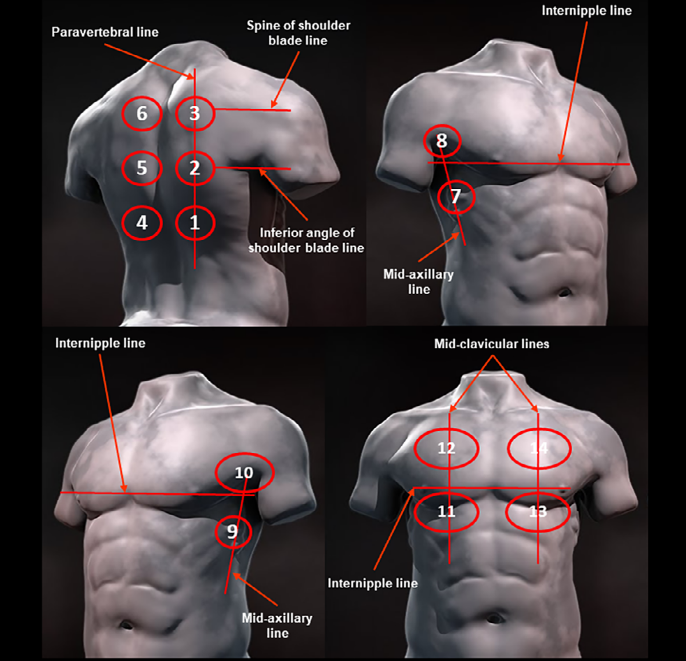
\includegraphics[width=0.5\linewidth]{images/us_protocols/14-points-protocol.png}
    \caption{The 14-points protocol proposed by Soldati et al.}
    \label{fig:us_protocols:soldati_protocol}
\end{figure}